\subsection{Connect \itwoc adapter to DCB data GBTxs}
\label{sec:dcb-data-i2c}
\itwoc adapter can be connected to the DCB mainboard directly, so that all 6
data GBTxs can be accessed via \itwoc.
Note that a FFC breakout board \emph{is still required} in this case, as no
ground connector is present on the mainboard and must be connected to any of the
4 FFC breakout boards.
Follow \autoref{fig:dcb-data-i2c} to connect an external \itwoc
adapter\footnote{
    As a reminder, in UMD, \itwoc adapter color coding is:
    yellow $\rightarrow$ \texttt{I2C SCL};
    blue $\rightarrow$ \texttt{I2C SDA};
}.

\begin{figure}[!ht]
\centering
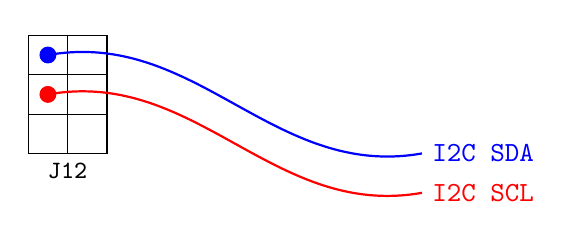
\begin{tikzpicture}
    % Pins
    \draw (0,0) rectangle (0.5,0.5);
    \draw (0.5,0) rectangle (1,0.5);

    \draw (0,-0.5) rectangle (0.5,0);
    \draw (0.5,-0.5) rectangle (1,0);

    \draw (0,-1) rectangle (0.5,-0.5);
    \draw (0.5,-1) rectangle (1,-0.5);

    % Helper labels (imaginary)
    \coordinate (B) at (0.5,-1);
    \node at (B) [below] {\small\texttt{J12}};

    % I2C SCL
    \draw [red,fill] (0.25,-0.25) circle [radius=0.1];
    \draw [red,thick] (0.25,-0.25)
        to [out=10,in=190] (5,-1.5) node [right] {\texttt{I2C SCL}};

    % I2C SDA
    \draw [blue,fill] (0.25,0.25) circle [radius=0.1];
    \draw [blue,thick] (0.25,0.25)
        to [out=10,in=190] (5,-1) node [right] {\texttt{I2C SDA}};
\end{tikzpicture}
\caption{
    \itwoc adapter can be connected on the DCB mainboard to access all 6 data
    GBTxs.
    Also note that no \texttt{GND} is present thus FFC breakout board is still
    required.
}
\label{fig:dcb-data-i2c}
\end{figure}
